\documentclass[]{article}
\usepackage{lmodern}
\usepackage{amssymb,amsmath}
\usepackage{ifxetex,ifluatex}
\usepackage{fixltx2e} % provides \textsubscript
\ifnum 0\ifxetex 1\fi\ifluatex 1\fi=0 % if pdftex
  \usepackage[T1]{fontenc}
  \usepackage[utf8]{inputenc}
\else % if luatex or xelatex
  \ifxetex
    \usepackage{mathspec}
  \else
    \usepackage{fontspec}
  \fi
  \defaultfontfeatures{Ligatures=TeX,Scale=MatchLowercase}
\fi
% use upquote if available, for straight quotes in verbatim environments
\IfFileExists{upquote.sty}{\usepackage{upquote}}{}
% use microtype if available
\IfFileExists{microtype.sty}{%
\usepackage{microtype}
\UseMicrotypeSet[protrusion]{basicmath} % disable protrusion for tt fonts
}{}
\usepackage[margin=1in]{geometry}
\usepackage{hyperref}
\hypersetup{unicode=true,
            pdftitle={CM 2.1 - Simple linear regression - SOLUTIONS},
            pdfborder={0 0 0},
            breaklinks=true}
\urlstyle{same}  % don't use monospace font for urls
\usepackage{color}
\usepackage{fancyvrb}
\newcommand{\VerbBar}{|}
\newcommand{\VERB}{\Verb[commandchars=\\\{\}]}
\DefineVerbatimEnvironment{Highlighting}{Verbatim}{commandchars=\\\{\}}
% Add ',fontsize=\small' for more characters per line
\usepackage{framed}
\definecolor{shadecolor}{RGB}{248,248,248}
\newenvironment{Shaded}{\begin{snugshade}}{\end{snugshade}}
\newcommand{\AlertTok}[1]{\textcolor[rgb]{0.94,0.16,0.16}{#1}}
\newcommand{\AnnotationTok}[1]{\textcolor[rgb]{0.56,0.35,0.01}{\textbf{\textit{#1}}}}
\newcommand{\AttributeTok}[1]{\textcolor[rgb]{0.77,0.63,0.00}{#1}}
\newcommand{\BaseNTok}[1]{\textcolor[rgb]{0.00,0.00,0.81}{#1}}
\newcommand{\BuiltInTok}[1]{#1}
\newcommand{\CharTok}[1]{\textcolor[rgb]{0.31,0.60,0.02}{#1}}
\newcommand{\CommentTok}[1]{\textcolor[rgb]{0.56,0.35,0.01}{\textit{#1}}}
\newcommand{\CommentVarTok}[1]{\textcolor[rgb]{0.56,0.35,0.01}{\textbf{\textit{#1}}}}
\newcommand{\ConstantTok}[1]{\textcolor[rgb]{0.00,0.00,0.00}{#1}}
\newcommand{\ControlFlowTok}[1]{\textcolor[rgb]{0.13,0.29,0.53}{\textbf{#1}}}
\newcommand{\DataTypeTok}[1]{\textcolor[rgb]{0.13,0.29,0.53}{#1}}
\newcommand{\DecValTok}[1]{\textcolor[rgb]{0.00,0.00,0.81}{#1}}
\newcommand{\DocumentationTok}[1]{\textcolor[rgb]{0.56,0.35,0.01}{\textbf{\textit{#1}}}}
\newcommand{\ErrorTok}[1]{\textcolor[rgb]{0.64,0.00,0.00}{\textbf{#1}}}
\newcommand{\ExtensionTok}[1]{#1}
\newcommand{\FloatTok}[1]{\textcolor[rgb]{0.00,0.00,0.81}{#1}}
\newcommand{\FunctionTok}[1]{\textcolor[rgb]{0.00,0.00,0.00}{#1}}
\newcommand{\ImportTok}[1]{#1}
\newcommand{\InformationTok}[1]{\textcolor[rgb]{0.56,0.35,0.01}{\textbf{\textit{#1}}}}
\newcommand{\KeywordTok}[1]{\textcolor[rgb]{0.13,0.29,0.53}{\textbf{#1}}}
\newcommand{\NormalTok}[1]{#1}
\newcommand{\OperatorTok}[1]{\textcolor[rgb]{0.81,0.36,0.00}{\textbf{#1}}}
\newcommand{\OtherTok}[1]{\textcolor[rgb]{0.56,0.35,0.01}{#1}}
\newcommand{\PreprocessorTok}[1]{\textcolor[rgb]{0.56,0.35,0.01}{\textit{#1}}}
\newcommand{\RegionMarkerTok}[1]{#1}
\newcommand{\SpecialCharTok}[1]{\textcolor[rgb]{0.00,0.00,0.00}{#1}}
\newcommand{\SpecialStringTok}[1]{\textcolor[rgb]{0.31,0.60,0.02}{#1}}
\newcommand{\StringTok}[1]{\textcolor[rgb]{0.31,0.60,0.02}{#1}}
\newcommand{\VariableTok}[1]{\textcolor[rgb]{0.00,0.00,0.00}{#1}}
\newcommand{\VerbatimStringTok}[1]{\textcolor[rgb]{0.31,0.60,0.02}{#1}}
\newcommand{\WarningTok}[1]{\textcolor[rgb]{0.56,0.35,0.01}{\textbf{\textit{#1}}}}
\usepackage{graphicx,grffile}
\makeatletter
\def\maxwidth{\ifdim\Gin@nat@width>\linewidth\linewidth\else\Gin@nat@width\fi}
\def\maxheight{\ifdim\Gin@nat@height>\textheight\textheight\else\Gin@nat@height\fi}
\makeatother
% Scale images if necessary, so that they will not overflow the page
% margins by default, and it is still possible to overwrite the defaults
% using explicit options in \includegraphics[width, height, ...]{}
\setkeys{Gin}{width=\maxwidth,height=\maxheight,keepaspectratio}
\IfFileExists{parskip.sty}{%
\usepackage{parskip}
}{% else
\setlength{\parindent}{0pt}
\setlength{\parskip}{6pt plus 2pt minus 1pt}
}
\setlength{\emergencystretch}{3em}  % prevent overfull lines
\providecommand{\tightlist}{%
  \setlength{\itemsep}{0pt}\setlength{\parskip}{0pt}}
\setcounter{secnumdepth}{0}
% Redefines (sub)paragraphs to behave more like sections
\ifx\paragraph\undefined\else
\let\oldparagraph\paragraph
\renewcommand{\paragraph}[1]{\oldparagraph{#1}\mbox{}}
\fi
\ifx\subparagraph\undefined\else
\let\oldsubparagraph\subparagraph
\renewcommand{\subparagraph}[1]{\oldsubparagraph{#1}\mbox{}}
\fi

%%% Use protect on footnotes to avoid problems with footnotes in titles
\let\rmarkdownfootnote\footnote%
\def\footnote{\protect\rmarkdownfootnote}

%%% Change title format to be more compact
\usepackage{titling}

% Create subtitle command for use in maketitle
\providecommand{\subtitle}[1]{
  \posttitle{
    \begin{center}\large#1\end{center}
    }
}

\setlength{\droptitle}{-2em}

  \title{CM 2.1 - Simple linear regression - SOLUTIONS}
    \pretitle{\vspace{\droptitle}\centering\huge}
  \posttitle{\par}
  \subtitle{Math 530/630}
  \author{}
    \preauthor{}\postauthor{}
    \date{}
    \predate{}\postdate{}
  

\begin{document}
\maketitle

{
\setcounter{tocdepth}{2}
\tableofcontents
}
\hypertarget{overview}{%
\section{Overview}\label{overview}}

\begin{itemize}
\tightlist
\item
  A complete knitted \texttt{html} file is due on Sakai by end of class
  Tuesday July 17th (before 5pm).
\item
  This lab is estimated to take approximately 45 minutes. We'll work
  together in chunks to keep tabs on time, with the aim that we all
  \emph{finish} during the in-class work period.
\item
  This lab is based on
  \href{http://moderndive.netlify.com/6-regression.html}{Chapter 6:
  Basic Regression in ModernDive}. Please open it and follow closely!
\item
  You'll need to load these packages to do the lab (make sure they are
  installed first, not in your .Rmd file!):
\end{itemize}

\begin{Shaded}
\begin{Highlighting}[]
\KeywordTok{library}\NormalTok{(moderndive)}
\KeywordTok{library}\NormalTok{(tidyverse)}
\KeywordTok{library}\NormalTok{(skimr)}
\end{Highlighting}
\end{Shaded}

\hypertarget{the-data}{%
\section{The data}\label{the-data}}

Source: John Clay (1856). ``On the Relation Between Crime, Popular
Instruction, Attendance on Religious Worship, and Beer-Houses'', Journal
of the Statistical Society of London, Vol. 20 \#1, pp 22-32.

In 1856, the Reverend John Clay felt that it was high time to figure out
what societal factors were playing a role in the incidence of criminal
behavior in Britain. He stated that:

\begin{quote}
``It is a mere truism to say that the progress of popular education, and
the formation of religious habits, are fatally opposed by the
temptations to animal pleasures, which abound wherever BEER-HOUSES and
low ALE-HOUSES abound.''
\end{quote}

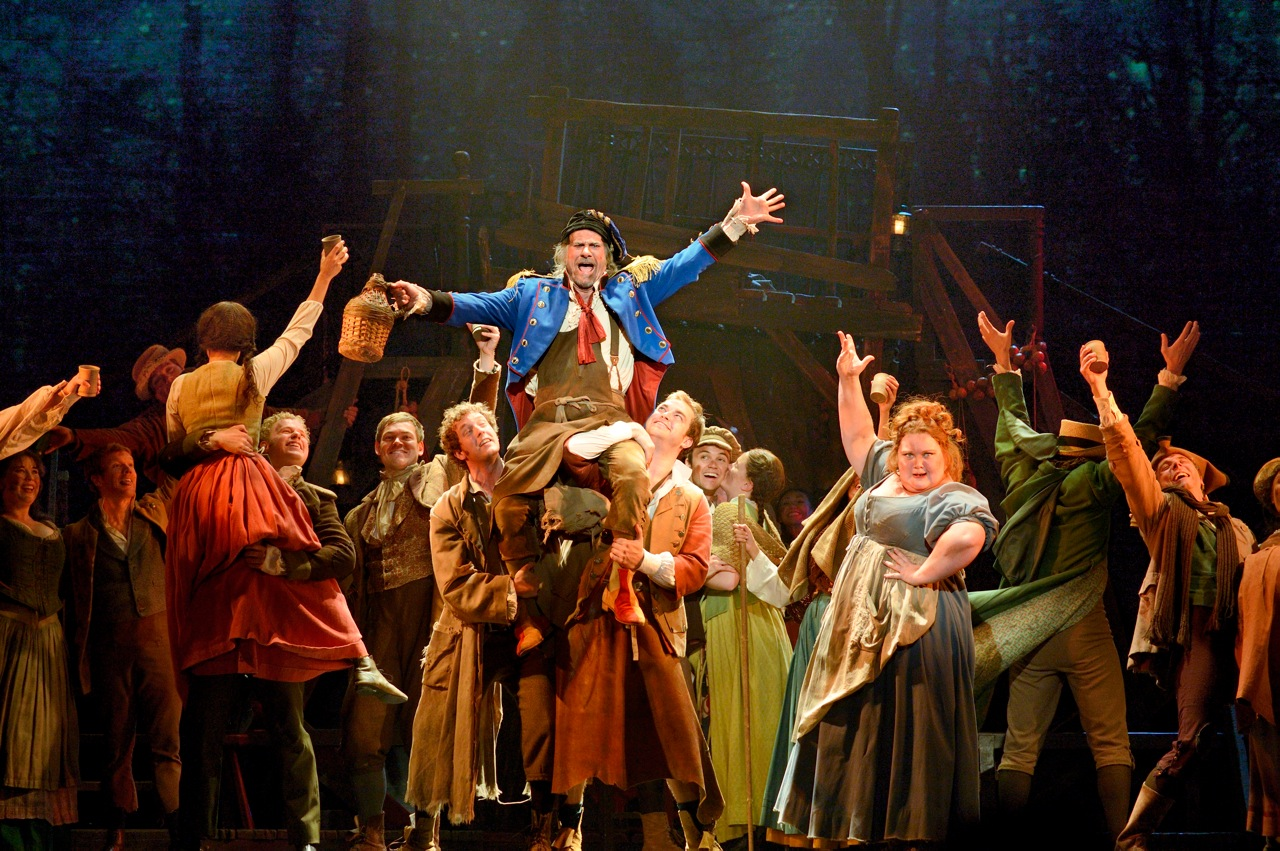
\includegraphics{../images/03.LesMiserables.US.MasteroftheHouse.jpg}

Clearly, the reverend considered public houses in Britain to be a
scourge on society, namely that they ``promote drunkenness and its
consequent evil'' (i.e., crime). Let's investigate how well we can
predict criminals (per 100k population) from the number of public houses
(ale/beer houses per 100k population) using simple linear regression.
Here is how to read in the data (please copy and paste into a code chunk
in your .Rmd):

\begin{Shaded}
\begin{Highlighting}[]
\NormalTok{crimenames <-}\StringTok{ }\KeywordTok{c}\NormalTok{(}\StringTok{"county"}\NormalTok{, }\StringTok{"region_name"}\NormalTok{, }\StringTok{"region_code"}\NormalTok{,}
               \StringTok{"criminals"}\NormalTok{, }\StringTok{"public_houses"}\NormalTok{, }\StringTok{"school_attendance"}\NormalTok{,}
               \StringTok{"worship_attendance"}\NormalTok{)}

\NormalTok{crime <-}\StringTok{ }\KeywordTok{read_table}\NormalTok{(here}\OperatorTok{::}\KeywordTok{here}\NormalTok{(}\StringTok{"data"}\NormalTok{, }\StringTok{"beerhall.dat"}\NormalTok{),}
                    \DataTypeTok{col_names =}\NormalTok{ crimenames)}
\end{Highlighting}
\end{Shaded}

\hypertarget{basics}{%
\section{Basics}\label{basics}}

Note: you don't need to use R to answer these questions, but please
create a section header using markdown format (\texttt{\#\ Basics}) and
type your answers there.

\begin{itemize}
\tightlist
\item
  What is the dependent variable? \texttt{criminals}
\item
  What is the independent variable? \texttt{public\_houses}
\item
  Copy and paste the provided equation that starts/ends with
  \texttt{\$\$} into your narrative (not an R code chunk), and replace
  \texttt{y} and \texttt{x} in this formula with meaningful variable
  names (you may wish to reference the \texttt{crimenames} object we
  made above):
  \texttt{\$\$\textbackslash{}hat\{y\}\ =\ b\_0\ +\ b\_1\{x\}\$\$}
\end{itemize}

\[\hat{\textrm{criminals}} = b_0 + b_1{\textrm{public_houses}}\]

\begin{itemize}
\tightlist
\item
  The ``best-fitting'' regression line is ``best'' in that it minimizes
  what?

  \begin{itemize}
  \tightlist
  \item
    Make sure you read
    \href{http://moderndive.netlify.com/6-regression.html\#leastsquares}{this}
  \end{itemize}
\end{itemize}

\begin{quote}
The best-fitting regression is one that minimizes the sum of the squared
residuals. Squared residuals are calculated by taking the difference
between the observed y values (here, criminals) and the fitted or
predicted y values (so y hat!), then squaring each of those differences.
The differences are squared so that positive and negative deviations of
the same amount are treated equally.
\end{quote}

\begin{itemize}
\tightlist
\item
  Why is this method called ``simple linear regression'' (as opposed to
  the method in
  \href{http://moderndive.netlify.com/7-multiple-regression.html}{Chapter
  7})?
\end{itemize}

\begin{quote}
Linear regression refers to the form of the statistical model we are
using- in linear regression, our model is in the form of a line, defined
by an intercept and slope. The ``simple'' part refers to the fact that
we have only one predictor variable (or independent variable/IV). In
multiple regression, we'll have two or more predictor variables or IVs.
All of these cases of regression are univariate, as opposed to
multivariate. Univariate vs.~multivariate refers to the number of
dependent variables or DVs. In this case, we just want to predict one
variable (here, \texttt{criminals}). In this course we will not cover
multivariate methods.
\end{quote}

\hypertarget{eda}{%
\section{EDA}\label{eda}}

Conduct a
\href{http://moderndive.netlify.com/6-regression.html\#model1EDA}{new
exploratory data analysis}, which involves three things:

\begin{itemize}
\tightlist
\item
  Looking at the raw values.
\item
  Computing summary statistics of the variables of interest.
\item
  Creating informative visualizations.
\end{itemize}

\hypertarget{look-at-the-data-all-together}{%
\subsection{Look at the data (all
together)}\label{look-at-the-data-all-together}}

Use \texttt{dplyr} to figure out how many counties are in this dataset,
and which variable names map onto the independent and dependent
variables you identified above.

\begin{Shaded}
\begin{Highlighting}[]
\KeywordTok{glimpse}\NormalTok{(crime)}
\end{Highlighting}
\end{Shaded}

\begin{verbatim}
Observations: 40
Variables: 7
$ county             <chr> "Middlesex", "Surrey", "Kent", "Sussex", "H...
$ region_name        <chr> "South Eastern", "South Eastern", "South Ea...
$ region_code        <dbl> 1, 1, 1, 1, 1, 1, 1, 1, 1, 1, 1, 1, 1, 2, 2...
$ criminals          <dbl> 200, 160, 160, 147, 178, 205, 183, 156, 173...
$ public_houses      <dbl> 541, 504, 552, 295, 409, 568, 708, 624, 463...
$ school_attendance  <dbl> 560, 630, 790, 820, 990, 930, 1020, 1130, 9...
$ worship_attendance <dbl> 434, 482, 680, 678, 798, 698, 888, 970, 848...
\end{verbatim}

\hypertarget{look-at-summary-statistics}{%
\subsection{Look at summary
statistics}\label{look-at-summary-statistics}}

Use \texttt{select} to select only the independent and dependent
variables you identified above, then pipe those variables to the
\texttt{skim} function from the \texttt{skimr} package (you should have
loaded this package at the top) to see summary statistics for each. Use
\texttt{dplyr::summarize} to calculate the correlation coefficient.

\begin{Shaded}
\begin{Highlighting}[]
\NormalTok{crime }\OperatorTok\StringTok{ }
\StringTok{  }\KeywordTok{select}\NormalTok{(criminals, public_houses) }\OperatorTok\StringTok{ }
\StringTok{  }\KeywordTok{skim}\NormalTok{()}
\end{Highlighting}
\end{Shaded}

\begin{verbatim}
Skim summary statistics
 n obs: 40 
 n variables: 2 

-- Variable type:numeric ----------------------------------------------------------------------------------------------------------------
      variable missing complete  n   mean     sd p0 p25   p50    p75 p100
     criminals       0       40 40 152.9   41.42 66 127 157.5 174.25  241
 public_houses       0       40 40 374.85 164.97 87 209 407   490.75  708
     hist
 <U+2582><U+2582><U+2583><U+2585><U+2587><U+2582><U+2583><U+2581>
 <U+2583><U+2586><U+2582><U+2582><U+2587><U+2585><U+2583><U+2582>
\end{verbatim}

\begin{Shaded}
\begin{Highlighting}[]
\NormalTok{crime }\OperatorTok\StringTok{ }
\StringTok{  }\KeywordTok{summarize}\NormalTok{(}\DataTypeTok{corr =} \KeywordTok{cor}\NormalTok{(criminals, public_houses))}
\end{Highlighting}
\end{Shaded}

\begin{verbatim}
# A tibble: 1 x 1
   corr
  <dbl>
1 0.463
\end{verbatim}

\hypertarget{visualize-the-data}{%
\subsection{Visualize the data}\label{visualize-the-data}}

Recreate the scatterplot below of ale/beer houses per 100K on the x-axis
and criminals per 100K population on the y-axis. What can you say about
the relationship between public houses and criminals based on this
exploration?

\begin{Shaded}
\begin{Highlighting}[]
\KeywordTok{ggplot}\NormalTok{(crime, }\KeywordTok{aes}\NormalTok{(}\DataTypeTok{x =}\NormalTok{ public_houses, }\DataTypeTok{y =}\NormalTok{ criminals)) }\OperatorTok{+}
\StringTok{  }\KeywordTok{geom_point}\NormalTok{() }\OperatorTok{+}
\StringTok{  }\KeywordTok{geom_smooth}\NormalTok{(}\DataTypeTok{method =} \StringTok{"lm"}\NormalTok{, }\DataTypeTok{se =} \OtherTok{FALSE}\NormalTok{)}
\end{Highlighting}
\end{Shaded}

\includegraphics{cm021-solutions_files/figure-latex/crime_scatterplot-1.pdf}

\begin{quote}
Do this in three sentences: There seems to be a moderately strong
relationship. The slope of the regresion line is positive, also the
correlation coefficient of 0.46 is moderate. Meaning as public houses
increase, there is an associated increase in criminal activity.
\end{quote}


\end{document}
